This chapter documents the implementation of the hardware and firmware of the \acrshort{tof} demonstrator.

All technical documents and some photos of the fabricated demonstrator are stored in the appendix~\ref{sec:schematic_apdx}
to and including~\ref{sec:apdx_photos_demonstrator}.

\subsection{Circuits}

In the following, all the sub-circuits that are necessary for the developed \acrshort{tof} evaluation module
are discussed. A complete schematic can be found in the appendix~\ref{sec:schematic_apdx}. The complete
project files are available in the electronic appendix of this project.

The schematic is drawn using the open-source tool \dq KiCad EDA 8.0\dq\ \cite{kicad2025kicadeda}.

\subsubsection{Selective Input Voltage}

Figure~\ref{fig:selective_input_voltage} shows the circuit for selecting the power supply.

\begin{figure}[H]
    \centering
    \includegraphics[page=2, trim=80 590 750 50, clip, width=0.9\textwidth]{../attachments/schematic.pdf}
    \caption{Selective Input Voltage}\label{fig:selective_input_voltage}
\end{figure}

The Nucleo board can be powered in the following ways:

\begin{itemize}
    \item 5~V from USB port
    \item 5~V from external power supply (\lstinline|JP1| + \lstinline|JP2|)
    \item 12~V from external power supply (\lstinline|JP3|)
\end{itemize}

See also chapter~\ref{sec:schematic_nucleo}.
The following options are available for supplying 5~V to the electronics:

\begin{itemize}
    \item 5~V from Nucleo board (\lstinline|JP1|)
    \item 5~V from external power supply (\lstinline|JP2|)
    \item 12~V from external power supply via Nucleo board (\lstinline|JP1| + \lstinline|JP3|)
\end{itemize}

The photodiode can be supplied with the following options:

\begin{itemize}
    \item 5~V from 5~V electronics (\lstinline|SW2| position 3)
    \item 12~V from an external power supply (\lstinline|SW2| Position 1)
\end{itemize}

See also chapter~\ref{sec:schematic_photo_receiver}.

\subsubsection{Nucleo Board}\label{sec:schematic_nucleo}

The circuitry of the NUCLEO-F042K6 board \cite{st2024nucleof042k6_usermanual} is shown in Figure~\ref{fig:nucleo_board}.

\begin{figure}[H]
    \centering
    \includegraphics[page=2, trim=530 580 300 50, clip, width=0.9\textwidth]{../attachments/schematic.pdf}
    \caption{Nucleo Board}\label{fig:nucleo_board}
\end{figure}

The NUCLEO board is a so-called \dq development kit\dq, which contains an STM32F042K6 \acrshort{mcu}.
Various pins of the \acrfull{mcu} are made available via pin headers at the edge of the board. This makes
the integration into your own electronics. The \acrshort{mcu} is flashed via an \acrshort{usb} interface.

In this design, the development board is also needed to operate the TDC7200 \acrshort{ic}s. For this purpose, a \acrfull{spi}
is used to configure and read the measurements (summarized as \acrshort{spi} bus in the figure).
With the signals \lstinline|start_ele| or \lstinline|start_opt| measurements can be started on the \acrshort{tdc}s. For
the \acrshort{tdc} that is responsible for the electrical signals, \lstinline|stop_ele| can also be used to
generate a stop pulse. Finally, the NUCLEO is responsible for controlling the laser diode, which is done with the
signals \lstinline|LD_pulse| and $\overline{\mbox{\lstinline|LD_enable|}}$

\subsubsection{TDC Electrical Signal}

The electrical circuit of the TDC7200 \cite{ti2016tdc7200_datasheet} for the electrical part is
shown in Figure~\ref{fig:tdc_ele_signal}.

\begin{figure}[H]
    \centering
    \includegraphics[page=2, trim=80 330 750 310, clip, width=0.9\textwidth]{../attachments/schematic.pdf}
    \caption{\acrshort{tdc} Electrical Signal}\label{fig:tdc_ele_signal}
\end{figure}

The TDC7200 is connected to the \acrshort{mcu} via the start and stop lines, an enable signal and the \acrshort{spi} lines.

As already mentioned in chapter~\ref{sec:approach}, the electrical \acrshort{tdc} is used to
to be put into operation for the first time and to familiarize yourself with it. At the \lstinline|J3| connection, a
cable of any length can be connected in a next step. This makes it possible to read the first measurement results, purely
electrically of course, from the TDC7200.

Using the switch \lstinline|SW1|, the \lstinline|STOP| signal can be generated either via \lstinline|stop_ele| or
\lstinline|start_ele|. This offers the possibility, on the one hand, to measure the time between the switching of two
\acrshort{gpio}s. On the other hand, the same \acrshort{gpio} pin can be used to generate the \lstinline|START| and
\lstinline|STOP| signals, which allows the delay time to be used to directly determine the cable length at \lstinline|J3|.

\subsubsection{TDC Optical Signal}

The circuitry of the TDC7200 \cite{ti2016tdc7200_datasheet} for the optical part is shown in Figure~\ref{fig:tdc_opt_signal}.

\begin{figure}[H]
    \centering
    \includegraphics[page=2, trim=530 330 300 310, clip, width=0.9\textwidth]{../attachments/schematic.pdf}
    \caption{\acrshort{tdc} Optical Signal}\label{fig:tdc_opt_signal}
\end{figure}

The \acrshort{tdc} is connected in practically the same way for the optical measurement as for the electrical
counterpart. The main difference here, however, is that the \lstinline|STOP| signal is not generated by the \acrshort{mcu}
itself, but by a comparator that is placed at the end of the optical measurement path. Since the comparator works with a
5~V level, the voltage divider \lstinline|R1| / \lstinline|R2| is needed to divide the 5~V pulse to the appropriate 3.3~V.

\subsubsection{Oscillator For TDCs}

The oscillator circuit for the two \acrshort{tdc} is shown in Figure~\ref{fig:oscillator_tdc}. It
is a normal quartz oscillator with an integrated oscillating circuit. Conveniently, this
means that no further circuitry is required.

\begin{figure}[H]
    \centering
    \includegraphics[page=2, trim=80 90 930 550, clip, width=0.45\textwidth]{../attachments/schematic.pdf}
    \caption{Oscillator for \acrshort{tdc}s}\label{fig:oscillator_tdc}
\end{figure}

\subsubsection{Power Supply Separation}

For the circuitry of the photodiode, including the \acrshort{tia} and comparator, it makes sense to have a power supply
with as little noise as possible.

For this purpose, the separation was carried out, which is shown in Figure~\ref{fig:power_supply_separation}.

\begin{figure}[H]
    \centering
    \includegraphics[page=2, trim=260 90 640 550, clip, width=0.7\textwidth]{../attachments/schematic.pdf}
    \caption{Power Supply Separation}\label{fig:power_supply_separation}
\end{figure}

In principle, the supplies should be somewhat suppressed by a ferrite bead. Of course, the
physical course of the supply path on the layout is also decisive here. More about this in the corresponding
chapter~\ref{sec:layout}. Alternatively, in addition to the ferrite beads, there is the option of further decoupling the
supply using capacitors. However, assumed that this is not necessary in a first step.

\subsubsection{Laser Driver}\label{sec:schematic_laser_driver}

The laser diode RLD65NZX1 \cite{rohm2019rld65nzx1_datasheet} is driven by a laser driver LMG1025-Q1
\cite{ti2024lmg1025q1_datasheet} and NexFET \cite{ti2016csd17578q3a_datasheet}. The AND gate \lstinline|IC21|
\cite{diodes202074lvc1g08q_datasheet} together with the high-pass filter (\lstinline|C21|, \lstinline|R21| and
\lstinline|RV21|) implements a pulse shortener. This path can be used to generate pulses in the range of 0.5
\dots 100~ns for the laser. See figure~\ref{fig:laser_driver}.

The resistor \lstinline|R25| forms the series resistor for the laser diode, which is calculated according to the
formula~\ref{eq:ld_resistor}.

\begin{equation}\label{eq:ld_resistor}
    R_{v} = \frac{V_{cc} - V_{fld}}{I_{ld}} = \frac{5~V - 2~V}{40~mA} = 75~\Omega
\end{equation}
\myequations{Laser diode series resistor}

A placeholder value is currently shown in the diagram. During commissioning, the resistance is. If it is reduced, the
current through the laser diode increases and thus the emitted light power.

\begin{figure}[H]
    \centering
    \includegraphics[page=3, trim=100 520 550 60, clip, width=0.9\textwidth]{../attachments/schematic.pdf}
    \caption{Laser Driver}\label{fig:laser_driver}
\end{figure}

\subsubsection{Photo Receiver}\label{sec:schematic_photo_receiver}

To amplify the photocurrent of the photodiode NJL6401R \cite{jrc2014njl6401r3_datasheet} and convert it into a voltage,
a transimpedance amplifier is built with the operational amplifier OPA858 \cite{ti2018opa858_datasheet}. The
output of the transimpedance amplifier goes to the comparator TLV3501 \cite{ti2016tlv3501_datasheet} to generate the
\lstinline|STOP| signal for the \acrshort{tdc}. See figure~\ref{fig:photo_receiver}.

The feedback resistor \lstinline|R26| can be changed as needed. Increasing it also increases the
negative pulse at the output of the \acrshort{tia}. With \lstinline|C20| a small capacitance can be added if needed.
This is to suppress oscillation of the amplifier, should it have a tendency to oscillate.

The offset of the OPA858 and the switching threshold of the TLV3501 can be adjusted using the two trimmers
\lstinline|RV22| and \lstinline|RV23|. This helps during commissioning, since it is not yet clear in advance where the
output of the operational amplifier will be due to the converted dark current of the photodiode.

\begin{figure}[H]
    \centering
    \includegraphics[page=3, trim=100 240 600 340, clip, width=0.9\textwidth]{../attachments/schematic.pdf}
    \caption{Photo Receiver}\label{fig:photo_receiver}
\end{figure}

\subsubsection{Decoupling Capacitors}

The circuitry of the decoupling capacitors is shown in figure~\ref{fig:decoupling_capacitors}. The capacitors for the
operational amplifier OPA858 and for the comparator TLV3501 are taken from the suggestion in the data sheet. In
addition, the gate driver at the laser driver is supported by an additional, larger capacity, which should have a
positive effect on the stability of the supply.

\begin{figure}[H]
    \centering
    \includegraphics[page=3, trim=100 60 650 630, clip, width=0.9\textwidth]{../attachments/schematic.pdf}
    \caption{Decoupling Capacitors}\label{fig:decoupling_capacitors}
\end{figure}

\pagebreak

\subsection{Layout}\label{sec:layout}

When laying out the circuit board, care is taken to ensure that the various circuits on the \acrshort{pcb} do not
interfere with each other. To this end, a clean power supply concept is used that defines the ground and power planes by
layer. In principle, the four layers of the circuit board are separated as follows:

\begin{itemize}
    \item Top layer: signal and ground
    \item Inner layer 1: power supply layer
    \item Inner layer 2: signal and ground
    \item Bottom layer: signal and ground
\end{itemize}

\begin{figure}[H]
    \centering
    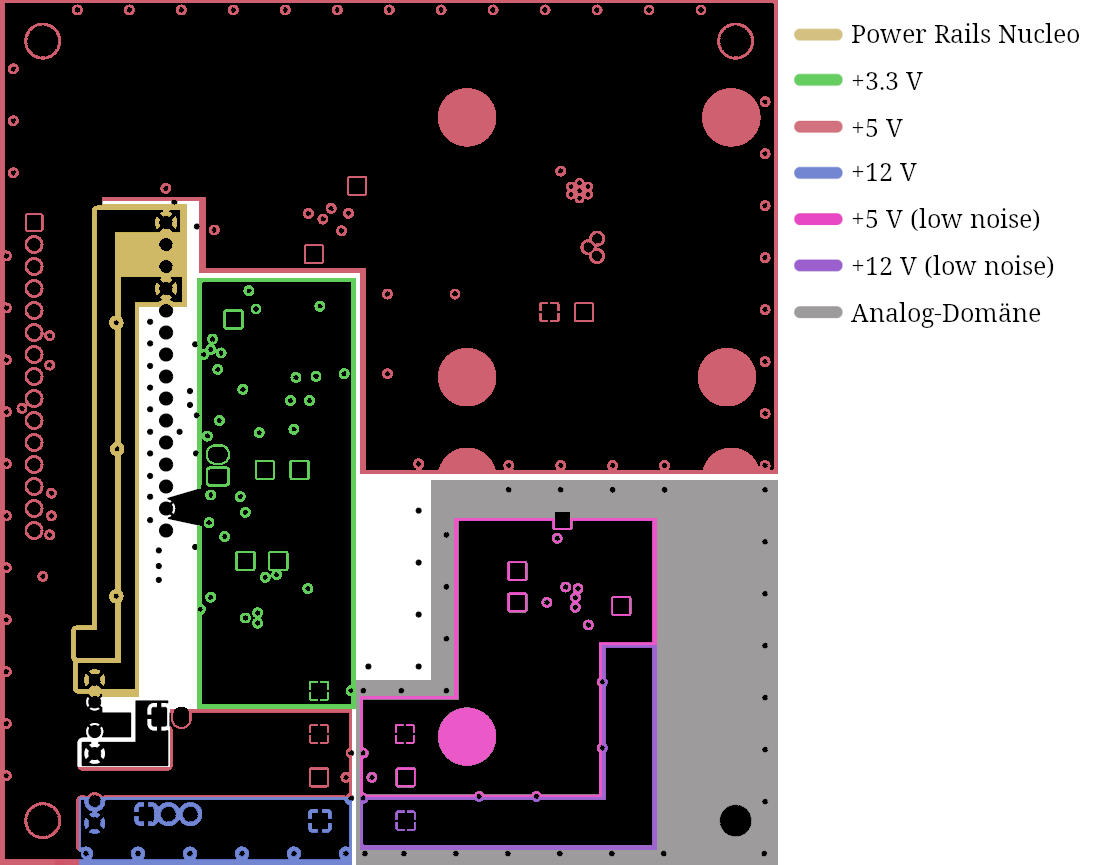
\includegraphics[width=0.9\textwidth]{../graphics/layout_annotated.png}
    \caption{Inner Layer 1 with notes on the supply concept}\label{fig:layout_annotated}
\end{figure}

Figure~\ref{fig:layout_annotated} shows the implementation of the supply concept. In the lower right corner
contains the photodiode, the \acrshort{tia} and the comparator. This section
of the \acrshort{pcb} has its own ground planes and suppressed power supplies. With the help of a few vias at the outer
boundary of this section, the analog domain should also be less susceptible to externally induced interference fields.

Such so-called \dq stitching vias\dq\ are also placed around the whole \acrshort{pcb} for shielding.

The complete layout can be found in the appendix~\ref{sec:apdx_layout}.

\pagebreak

\subsection{3D View}

A 3D view can be helpful when designing the layout and especially when placing components. This is because
it shows where mechanical and electronic components could get in each other's way. The figure~\ref{fig:3d_top}
shows a 3D rendering of the top view of the \acrshort{tof} demonstrator.

\begin{figure}[H]
    \centering
    
\includegraphics[width=0.5\textwidth]{../graphics/3d_top.png}
    \caption{3D View Top}\label{fig:3d_top}
\end{figure}

The lens mounts are integrated into the view using a step file provided by QIOPTIQ
\cite{qioptiq2024g061041000_shoppage}. In the figure~\ref{fig:3d_top}, these are shown as black cuboids with
cylindrical cutouts. There must be no components directly under these holders, as otherwise the holders cannot be mounted.

When placing the components, care is also taken to ensure that all test points, trimmers and
switches for configuration are easily accessible. If these components are close to the optoelectronic components,
they are placed on the underside. This means that they are also available with the optics mounted.

\subsection{Fabrication}

KiCad 8.0 allows you to create various manufacturing files for the different layers from the layout design.
These so-called Gerber and NC-Drill files can be used by a PCB manufacturer to produce a printed circuit board.
Optionally, a printed circuit board can also be assembled directly, but this takes additional time in
production.

Since most components can be mounted relatively easily on the \acrshort{pcb}, automated assembly is
avoided and the components are mounted by hand.

The components are ordered from Mouser Electronics, while the printed circuit boards are
\cite{jlc2025jlcpcb} obtained from the Chinese manufacturer JLCPCB. Mouser meets the expected delivery time of a few days.
The order from JLCPCB also arrives on time, exactly seven days later. JLCPCB's engineers do not need to ask any questions
about the design, which probably has a positive effect on the delivery time.

The finished printed circuit board can be seen in the figure~\ref{fig:photo_demonstrator_front_wo_lens}. Further
photographs of the \acrshort{tof} demonstrator can be found in the appendix~\ref{sec:apdx_photos_demonstrator}.

\begin{figure}[H]
    \centering
    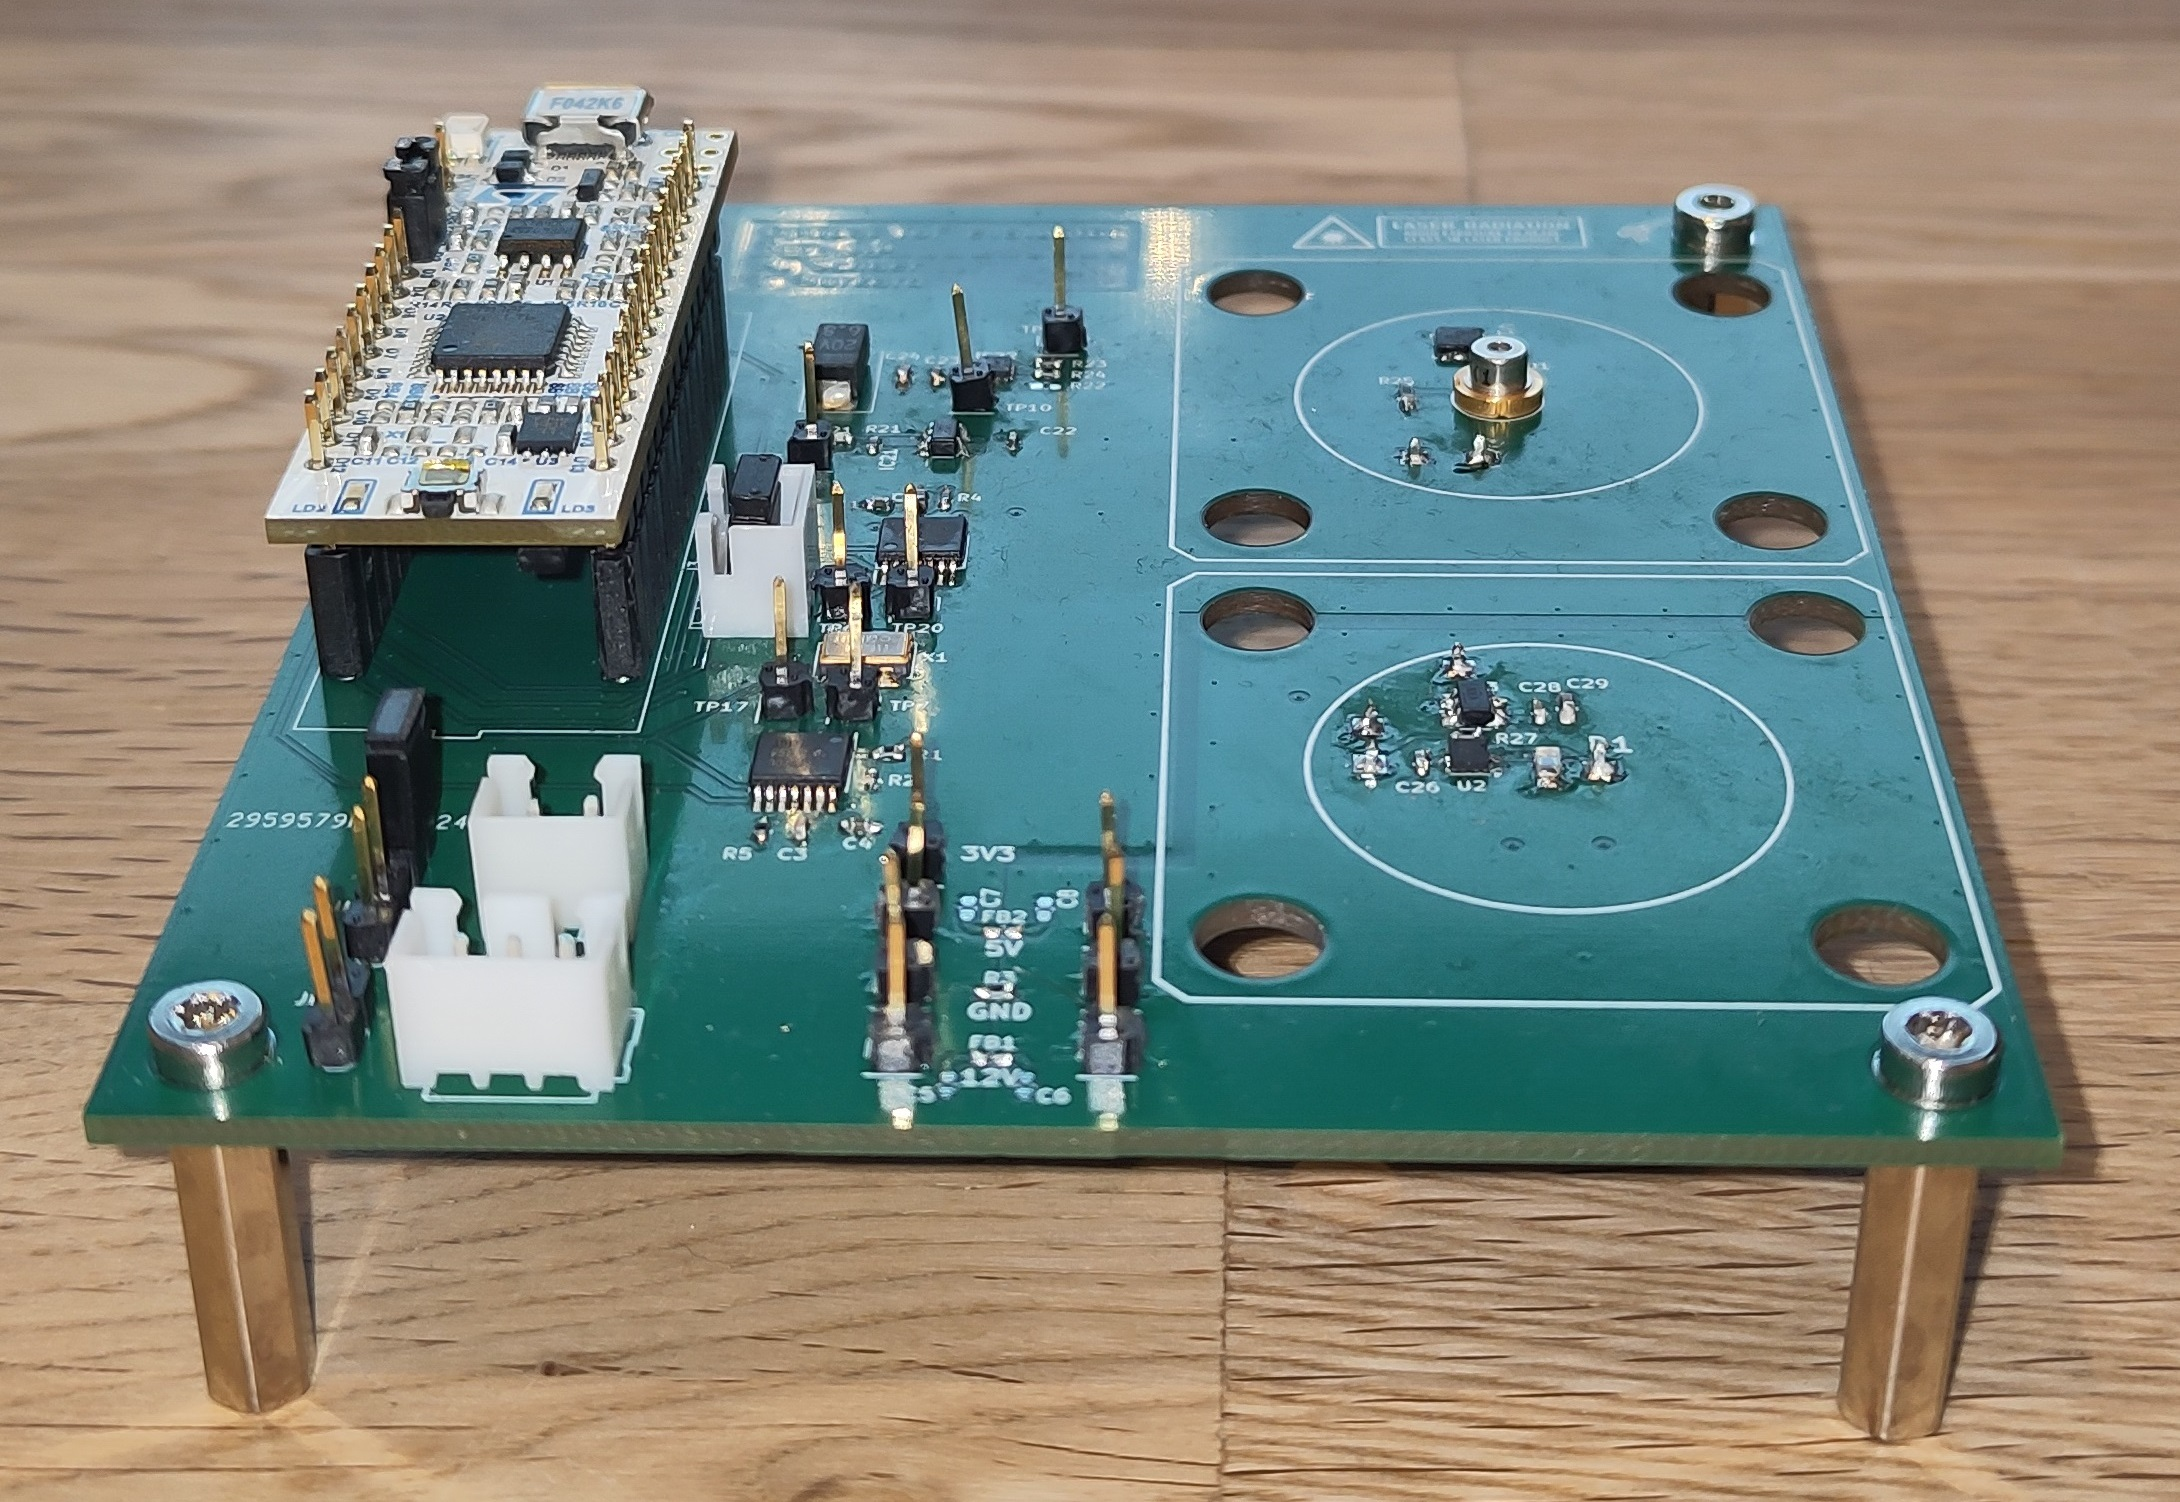
\includegraphics[width=0.6\textwidth]{../graphics/photo_demonstrator_front_wo_lens.jpg}
    \caption{Demonstrator from the front without lens}\label{fig:photo_demonstrator_front_wo_lens}
\end{figure}

\subsection{Firmware}

When it comes to the firmware, care is taken to ensure that there is a clean separation between the application, the
driver and the peripherals. This ensures that the design is as modular as possible. The \acrshort{fw} hierarchy is
Figure~\ref{fig:hierarchy_firmware} comprehensible.

\begin{figure}[H]
    \centering
    \includegraphics[width=0.5\textwidth]{../diagrams/Aufbau_FW.pdf}
    \caption{Structure of the firmware project}\label{fig:hierarchy_firmware}
\end{figure}

The application is responsible for the timing of the measurements. The code for triggering is expanded step by step
during the measurement phase, starting with the use of simple \acrshort{gpio}s, and ending with optimal timing behavior
using various hardware timers to generate the trigger pulses for the \acrshort{tdc}s. The individual expansion steps
are explained in more detail in chapter~\ref{sec:electrical_measurements}. explains the individual expansion steps in
more detail.

The \acrshort{tdc} driver provides functions for initializing and enabling the \acrshort{tdc}.
See code~\ref{code:init_enable_tdc} for an example.

\lstinputlisting[language={C}, label={code:init_enable_tdc}, caption={\acrshort{tdc} Init and Enable with Driver}]{../sourcecode/init_enable_tdc.c}

The \acrshort{tdc} driver contains the complete register definition of the TDC7200. The driver also provides simple
read and write routines for communication via \acrshort{spi}. This makes it easy to reconfigure, set up and read out the
measurement \acrshort{ic}. An example is shown in Code~\ref{code:read_write_tdc}.

\lstinputlisting[language={C}, label={code:read_write_tdc}, caption={\acrshort{tdc} Read/Write with Driver}]{../sourcecode/read_write_tdc.c}

Furthermore, the driver can directly convert the measurement results using the formulas given in the data sheet
formulas. The code~\ref{code:start_measurement_tdc} shows an example of code for a single measurement.

\lstinputlisting[language={C}, label={code:start_measurement_tdc}, caption={\acrshort{tdc} Measurement with driver}]{../sourcecode/example_tdc_read.c}

The self-developed firmware driver for the \acrshort{tdc} is in the appendix~\ref{sec:tdc_driver}.

With the development environment STM32CubeIDE / CubeMX \cite{st2025stm32cubeide}, it is possible to \acrshort{mcu} can
be configured graphically. With the help of a code generator, the initialization routines for all peripherals can be
generated automatically. This allows the focus to be placed on the \acrshort{tdc} driver and the actual application
during development.

The pin configuration can be seen in the figure~\ref{fig:pinconfiguration_mcu}.

\begin{figure}[H]
    \centering
    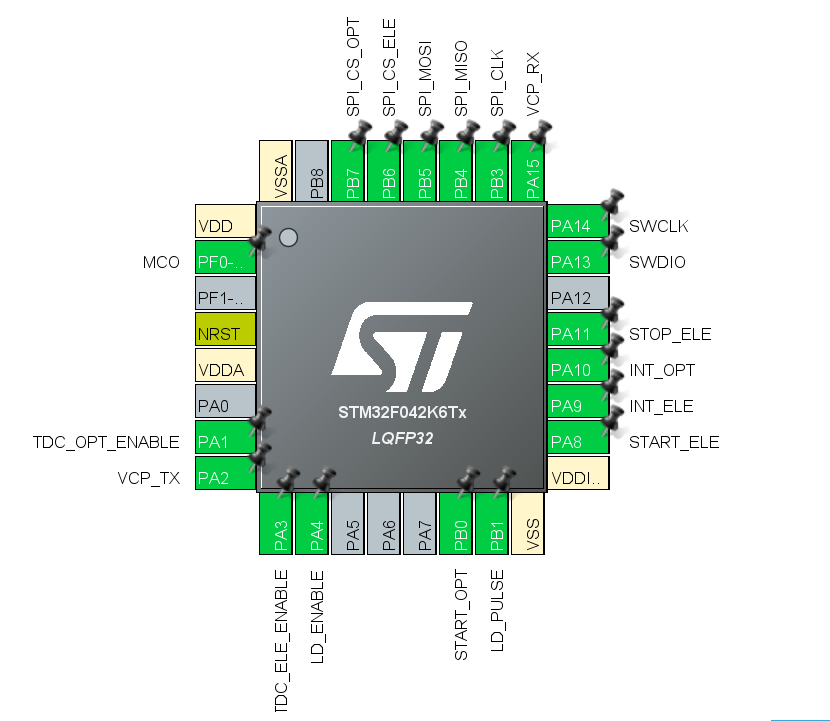
\includegraphics[width=0.6\textwidth]{../graphics/pinconfiguration_mcu.png}
    \caption{Pin configuration of the STM32F042K6}\label{fig:pinconfiguration_mcu}
\end{figure}

\pagebreak
